\documentclass[11pt]{article}
\usepackage{icmlko}
\begin{document}

\title{여섯 번 설명에 실패했다 --- 웹툰을 관측으로 둔다}
\author{월드모델 실험실}
\date{노트 414 · 2026년 8월 2일}
\maketitle

\begin{abstract}
이번 사이클에서 판을 움직인 기계 넷 --- 나무 깊이(노트 406) · 학습률
(노트 408) · 자루마다 깊이 섞기(노트 409) · 집단 표지 축 grp(노트 413) ---
에서 \textbf{웹툰이 네 번 다 혼자 음수 쪽에 있었다}. 넷 중 셋은 판을 올려
채택했거나 축을 확정했고, 그때마다 웹툰만 반대로 갔다.

웹툰은 유보 711행으로 \textbf{판 무게의 21\%} 다. 그래서 이 한 도메인이
전역 손잡이를 계속 끌어내린다 --- 깊이 8 이 막힌 것도(노트 412 관문에서
웹툰 $-0.0128$) 여기다.

설명을 여섯 번 시도했다.

\begin{center}
\begin{tabular}{llr}
\hline
후보 & 잰 값 & 결과 \\
\hline
크기 (유보 · 학습 행) & $\rho = -0.01$ & 죽음 \\
원핫 아쉬움 & $\rho = +0.37$ & 죽음 \\
표시자 무늬 순도 & $\rho = +0.07$ & 죽음 \\
비선형 요구 & $\rho = +0.77$ & \textbf{열한 중 열만} \\
학습--유보 시간 어긋남 & $\rho = +0.04$ & 죽음 \\
\textbf{보관함 835행} & $-0.0013 \to -0.0045$ & \textbf{죽음} \\
\hline
\end{tabular}
\end{center}

마지막 것이 이 노트의 새 측정이다. 이번 사이클에 웹툰 학습에 넣은
\textbf{보관함 835행}(전부 2025년 이전이라 유보는 안 건드린다)이 원인인가.
사전 등록했다 --- \emph{빼면 깊이 반응이 양수로 돌아서거나 크게 덜 음수가
된다.}

\textbf{반대로 갔다.} 빼니 깊이 반응이 $-0.0013 \to \mathbf{-0.0045}$ 로
\textbf{더 음수}가 됐다. 보관함 행은 원인이 아니고 오히려 조금 눅인다.
(덤: 보관함은 웹툰 자체에 $+0.0091$ 로 이롭다 --- 이번 사이클의 채택이
옳았다.)
\end{abstract}

\section{관측으로 둔다}

노트 385가 달력에 대해 한 것과 같은 처분이다 --- 설명 넷이 실패했을 때
``관측으로 둠''이라 적고 넘어갔다. 여기서는 여섯이다.

남는 것은 사실 자체다: \textbf{용량을 늘리는 어떤 조작에도 웹툰은 조금씩
잃는다.} 비선형 요구는 넷째로 갖고 있는데($+0.1050$) 용량 선호는 열째다
($+0.0020$). 노트 410의 축이 열한 중 \textbf{열}을 설명하고 이 하나만
남는다 --- 잔차가 $-6.0$ 인데 나머지 열은 전부 $\pm 2$ 안이다.
\textbf{두 번째 축이 아니라 한 점짜리 예외다.}

\section{정렬 검사가 한 번 살렸다}

이 측정은 행 순서로 마스크를 만든다 --- 보관함 835개의 레코드 번호를
판의 행에 맞춰야 한다. 그래서 \textbf{연도 대조}를 안전 장치로 먼저 넣었고,
처음에 \textbf{일치율 $0.4997$} 이 나와 스크립트가 스스로 멈췄다.

원인은 자료가 아니라 \textbf{검사 쪽}이었다 --- 판의 \texttt{yr} 은
\emph{소수 연도}($2020.834 \leftrightarrow$ 2020-11-01)인데 레코드의
연도(정수)와 $\pm 0.51$ 로 견줬으니 \textbf{7월 이후에 시작한 작품이 전부
불일치}로 세어졌다. 정확히 절반이 나온 것이 단서였다. \texttt{floor} 로
고치니 $0.9989$ 다.

검사가 틀렸는데도 값을 했다. \textbf{안 넣었으면 절반이 어긋난 마스크로
835행을 지우고 그 결과를 믿었을 것이다.}

\section{남은 것}

\begin{tabular}{lp{7.2cm}}
\hline
웹툰 & \textbf{관측으로 둔다.} 여섯 번 실패. 판 무게 21\% 라 대가는 계속
치른다 \\
웹툰을 쪼개 볼까 & 3{,}652행이 한 도메인인 것이 맞나 --- 유일하게 안 해 본
방향이다 \\
전용 축의 통로 & 시장팝업 $+0.0241$(노트 412)은 아직 갈 곳이 없다 \\
\hline
\end{tabular}

\begin{figure}[h]
\centering
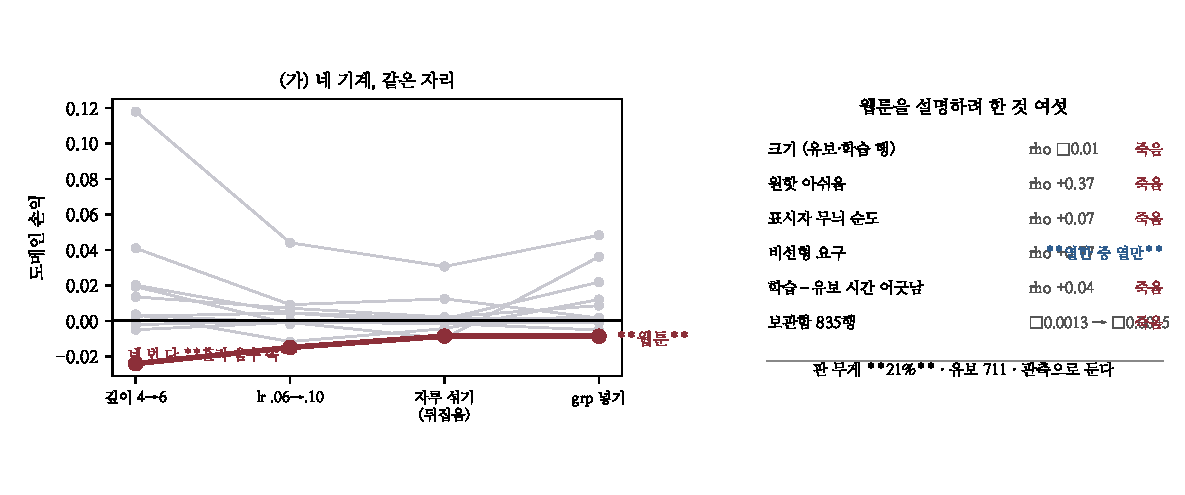
\includegraphics[width=\textwidth]{figs/fig414.pdf}
\caption{(가) 판을 움직인 기계 넷에서 웹툰(붉은 굵은 선)만 네 번 다 음수
쪽. (나) 여섯 후보와 그 결과.}
\end{figure}

\end{document}
